\chapter{Introduction}

This report describes an implementation of the classic two player game PONG using an HCS12 microprocessor and a serial controlled, OLED (organic light emitting diode) screen.
Chapter \ref{ch:support} describes various functionality required by the project including an overview of the methods used to control the OLED.
A description of the techniques used in communication between the HCS12 and OLED, as well as the method used to create pseudrandom numbers, and an overview of techniques which allow C and assembly code to be used in tandem is also presented.
Chapter \ref{ch:pong} contains details of the PONG program itself, including how the players' paddles and the ball are moved and controlled, and how the LCD (liquid crystal display) is used to display a scores.
Finally, a complete listing of source code is presented in appendix \ref{ch:code}.

\section{Rules and Game Objectives}

The rules of this game are quite simple, and very similar to the original PONG's.
Two players, using buttons, are able to move rectangular \q{paddles} on the OLED screen.
Movement is constrained in the vertical direction, within the bounds of the screen.
A ball bounces between the two paddles.
The ball begins in the center of the screen, and begins moving in a pseudorandomly selected direction, continuing to move in the along the same vector until it reaches either the top or bottom of the screen, which cause it to assume the opposite velocity in the y-direction; or either the left or right side of the screen, which causes the player whose paddle is on the opposite side to the screen to have scored a point.
Either player may reflect the ball, using their paddle, by having the ball come into contact with the paddle, causing the ball to take on a pseudorandom velocity in the opposite x-direction.
The game objective of each player, scoring on their opponent is tracked on the LCD screen on the Dragon12 board.

\section{System Components}

The figure below illustrates the basic configuration of the system used in this project, which is an integrated 'Dragon12' board consisting of an HCS12 microprocessor, with a variety of other hardware.
One of the integrated devices on the Dragon12 is an LCD directly connected to a digital I/O port of the microprocessor.
It consists of two-lines of alphanumeric text and is used to display the current score.
A full color, 320 by 240 pixel OLED external to the Dragon12 board was connected to another one of the microprocessor's digital I/O ports, and communicates with it via RS232 protocol, for the purpose of serving as the game display.

\begin{figure}[htp]
    \centering
    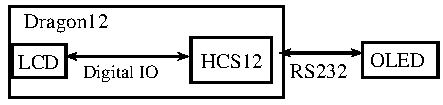
\includegraphics[width=.6\textwidth]{images/SystemDiagram.pdf}
    \caption{System Diagram}
    \label{fig:sysdiag}
\end{figure}